\section{Innovations In Vapor Intrusion Investigations}

In an attempt to reduce the uncertainty in determining human exposure due to vapor intrusion caused by the significant spatial and temporal variability in VI, a number of new investigatory techniques and methods have been proposed, but in general their efficacy is yet to be fully established\cite{mchugh_recent_2017}.
This work won't deal with all of these exhaustively, but rather primarily address two approaches (together with other topics related to variability.)\par

\subsection{Controlled Pressure Method}

Most buildings are naturally depressurized relative to atmosphere due to the operation of heating, ventilation, and air conditioning systems, and the so-called stack effect, a topic that will be covered in greater detail in Chapter \ref{chp:transport_implications}.
This depressurization induces a flow of air from soil into the building; this flow can carry contaminant vapors into the building.
(This view is rather simplistic, as will be discussed throughout this work, but suffices for now.)
Using this idea, the controlled pressure method (CPM) was suggested, where blowers are used to control the depressurization of the building, and thereby more effectively control the indoor environment (see Figure \ref{fig:cpm_cartoon}).
The basic ideas was to create a "worst case" scenario in which contaminant soil vapors are induced to enter the building.\par

\begin{figure}[htb!]
  \centering
  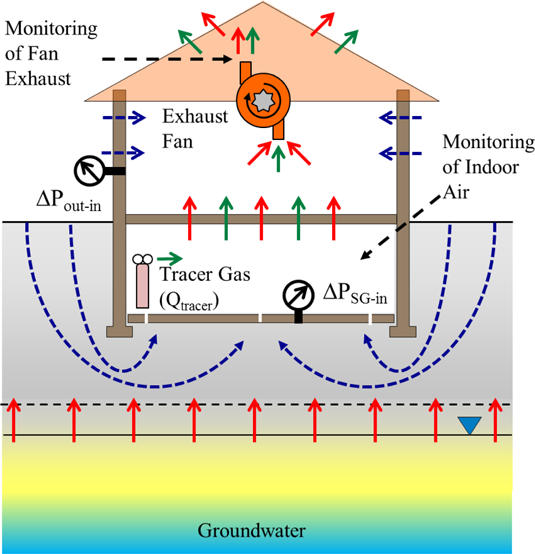
\includegraphics[width=0.75\textwidth]{cpm_cartoon.jpg}
  \caption[Overview of the controlled pressure method concept]{Conceptual idea of the controlled pressure method - a VI impacted building is forcefully pressurized using a blow, theoretically controlling the contaminant entry into the building. Figure from \citeauthor{holton_long-term_2015}\cite{holton_long-term_2015}.}
  \label{fig:cpm_cartoon}
\end{figure}

Within the CPM framework, overpressurizing a building will then prevent contaminant entry from occurring.
Thus, this can be used to identify indoor contaminant sources, as the presence of any contaminant vapors in the indoor environment in the overpressurized building have to originate from such a source.
This approach can be applied as needed and hopefully will reduce the uncertainty and difficulty of VI investigations\cite{mchugh_evaluation_2012}.\par

\subsection{Indicators, Tracers, and Surrogates}

The conventional sampling schemes currently employed, due to the spatial and temporal variability of VI, has a propensity for creating false positives and negatives.
While one solution to this problem is to increase the scope of VI investigations of a particular site, by for instance continuously monitoring the indoor contaminant concentration or by collecting an increasing number of samples, this approach is not practical, especially when numerous sites are involved.
Thus, there is a need to develop guidelines that help reduce the sampling requirements and scope of VI investigations, while retaining the same degree of confidence that the relevant level of VI has been determined\cite{schuver_chlorinated_2018}.\par

To achieve this, it has been suggested to use indicators, surrogates, and tracers (ITS) to determine when to conduct a VI site investigation.
For example, one question that has been posed is if meteorological ITS be used to determine when VI is expected to be the greatest, e.g. at which temperature and barometric pressure is, for instance, the \nth{95} percentile indoor contaminant concentration most likely to be found\cite{schuver_chlorinated_2018}?
This is a promising approach, because as we have already discussed, many VI sites have the highest indoor contaminant concentration during colder seasons.
So far this is more of a qualitative observation rather than quantitative guidelines for use in VI site investigations.\par
